\documentclass[../main.tex]{subfiles}

\begin{document}

\chapter{Results} \label{chapter:results}

This chapter presents the results of each experiment proposed in chapter \ref{chapter:methodology}. In all tables and graphs shown below, the precision, recall and F1 score metrics are expressed as real numbers between 0 and 1 with 3 decimal places.

\section{Research Question 1 Results}

Tables \ref{table:rq1_Precision}, \ref{table:rq1_Recall} and \ref{table:rq1_F1} provide a comparison between the performance of the  random forest and XGBoost models with previous benchmarks. The values for the \textbf{Kamei} and \textbf{Deeper} baselines were obtained from the paper \textit{Deep Learning for Just-In-Time Defect Prediction} \cite{yang2015deep} and the values for \textbf{TLEL} were obtained from \textit{TLEL: A two-layer ensemble learning approach for just-in-time defect prediction} \cite{yang2017tlel}.

\begin{table}[H] 
\centering 
\caption{Comparing precision to past results} 
\begin{tabular}{|c c c c c c c c c|} 
\hline 
Project  & Kamei& Deeper & TLEL  & LR & RF   & ADA    & XGB & KNN \\ 
\hline \hline 
Bugzilla & 0.548 & 0.556 & 0.624 & 0.539  & 0.583 & 0.568 & 0.586  & 0.497    \\ 
\hline 
Columba  & 0.487 & 0.469 & 0.512 & 0.490  &0.495  & 0.475 & 0.493  & 0.421  \\ 
\hline 
JDT      & 0.249 & 0.260 & 0.293 & 0.260  & 0.265 & 0.272 & 0.281  & 0.224     \\ 
\hline 
Mozilla  & 0.124 & 0.132 & 0.158 & 0.129  &0.148  & 0.136 & 0.149  & 0.095 \\ 
\hline 
Platform & 0.232 & 0.264 & 0.314 &  0.263  &0.294  & 0.284 & 0.296  & 0.236    \\ 
\hline 
Postgres & 0.504 & 0.457 & 0.499 & 0.497  &0.478  & 0.485 & 0.503  & 0.399     \\ 
\hline 
Average  & 0.357 & 0.356 & 0.400 & 0.363  & 0.377     &  0.370      & 0.385  &  0.312    \\ 
\hline 
\end{tabular} 
\label{table:rq1_Precision} 
\end{table} 

\begin{table}[H] 
\centering 
\caption{Comparing recall to past results} 
\begin{tabular}{|c c c c c c c c c|} 
\hline 
Project  & Kamei & Deeper & TLEL  & LR    & RF    & ADA   & XGB  & KNN\\ 
\hline \hline 
Bugzilla & 0.702 & 0.721  & 0.759 & 0.659 & 0.690 & 0.695 &0.697  & 0.656\\ 
\hline 
Columba  & 0.649 & 0.670  & 0.743 & 0.644 & 0.682 & 0.648 &0.694  & 0.636\\ 
\hline 
JDT      & 0.661 & 0.688  & 0.735 & 0.667 & 0.695 & 0.677 & 0.702  & 0.616\\ 
\hline 
Mozilla  & 0.608 & 0.682  & 0.778 & 0.639 & 0.738 &0.702  &0.740  & 0.685\\ 
\hline 
Platform & 0.709 & 0.700  & 0.775 & 0.691 & 0.718 & 0.713 & 0.738  & 0.665\\ 
\hline 
Postgres & 0.602 & 0.680  & 0.770 & 0.646 & 0.711 & 0.702 &0.707  & 0.629\\ 
\hline 
Average  & 0.655 & 0.690  & 0.760 & 0.658 & 0.706 & 0.690 & 0.713  & 0.648\\ 
\hline 
\end{tabular} 
\label{table:rq1_Recall} 
\end{table} 

\begin{table}[H] 
\centering 
\caption{Comparing F1 score to past results} 
\begin{tabular}{|c c c c c c c c c|} 
\hline 
Project  & Kamei & Deeper& TLEL  & LR    & RF   & ADA & XGB & KNN\\ 
\hline \hline 
Bugzilla & 0.615 & 0.626 & 0.685 & 0.592 &0.631 & 0.624 &0.635 & 0.564\\ 
\hline 
Columba  & 0.555 & 0.549 & 0.607 & 0.554 &0.572 & 0.547 &0.573&0.505\\ 
\hline 
JDT      & 0.362 & 0.377 & 0.419 & 0.373 &0.383 & 0.387 &0.401 &0.328\\ 
\hline 
Mozilla  & 0.206 & 0.221 & 0.263 & 0.215 &0.246 & 0.228 &0.248&0.168\\ 
\hline 
Platform & 0.350 & 0.383 & 0.447 & 0.381 &0.417 & 0.406 &0.422&0.348\\ 
\hline 
Postgres & 0.548 & 0.546 & 0.605 & 0.561 &0.571 & 0.573 &0.587&0.488\\ 
\hline 
Average  & 0.439 & 0.451 & 0.504 & 0.446 &0.470 & 0.461  &0.478 & 0.400\\ 
\hline 
\end{tabular} 
\label{table:rq1_F1} 
\end{table} 

Tables \ref{table:rq1_Precision} to \ref{table:rq1_F1} show that the choice of classification algorithm does make a significant impact on precision, recall and F1 score. Out of the five models chosen to experiment (LR to KNN), XGBoost performs the best overall. K-nearest neighbours on the other hand consistently underperforms when compared to the other models. Tables \ref{table:rq1_Precision} and \ref{table:rq1_Recall} show that in most cases, models tend to achieve higher values for the recall score as opposed to the precision score. 

When comparing to the previous benchmarks, decision tree based models such as random forest, Adaboost and XGBoost all outperform the deep learning model Deeper as well as the results obtained by Kamei et al. The benchmark model TLEL on the other hand performs the best out of all models. TLEL consists of two layers of random forest which can explain the higher performance as opposed to a single random forest model. 

The hardest project to achieve a high performance on is Mozilla which has the lowest F1 scores.  This is because the project's rate of buggy commits is only 5\%. Due to the severe imbalance, sampling techniques like undersampling have to be applied so that these models see roughly the same number of \textit{risky} commits as \textit{not risky} commits. However, undersampling deletes samples for the training set which could have been of value.

\section{Research Question 2 Results}

For this section, the result of running the evaluation algorithm (see algorithm \ref{algorithm:evaluation}) is summarized in tables and graphs. For some of the experiments, the performance of a random model is provided as an additional baseline in the column RAND. The values for a random model's performance are obtained by creating and running a model that returns randomized predictions as opposed to using the theoretical value of each metric. This is done to see if the theoretical value matches what is obtained in practice. For the purpose of confidentiality, the precision and F1 score of random models are not included for commercial projects as the percentage of risky commits can be derived using these values. 

\subsection{Experimenting with Five Models}\label{subsection:experiment1}

Tables \ref{table:rq2_exp1_Precision}, \ref{table:rq2_exp1_Recall} and \ref{table:rq2_exp1_F1} show the precision, recall and F1 score for each model when applied on all nine datasets. Each table cell has two values, one for the supervised model and another for its self-trained counterpart. The values in bold are those where the self-training algorithm made a statistically significant improvement over its respective base classifier. In all cases, these models manage to achieve higher than random performances which indicate that the models have found some connection between the provided features and whether or not a commit is risky. 

\subsubsection{Precision}

When it comes to self-training performance, the self-training algorithm does not appear to improve performance when both classifiers are provided the exact same amount of labelled data. As seein in table \ref{table:rq2_exp1_Precision}, K-nearest neighbours has the most benefit from self-training as seen for the JDT, Platform, Postgres, C2 and C3 projects. However, even with this increase, KNN is performing worse than the tree based models (RF, ADA, XGB). In most cases, the precision due to self-training is similar or slightly lower than the base performance. Also, the precision on the commercial projects happens to be higher, possibly due to a smaller class imbalance.



\begin{table}[H] 
 \centering 
  \caption{Precision for various models and datasets, bold value represents cases where self-training provides a statistically significant improvement over the base classifier} 
 \begin{tabular}{|p{15mm}p{15mm}p{15mm}p{15mm}p{15mm}p{15mm}P{15mm}|} 
 \hline 
Project &LR & RF & ADA & XGB & KNN & RAND\\ 
\hline \hline 
Bugzilla& 0.539 \newline 0.531 & 0.583 \newline 0.602 & 0.568 \newline 0.565 & 0.586 \newline 0.592 & 0.497 \newline 0.485 & 0.372 \\ 
\hline 
Columba& 0.490 \newline 0.496 & 0.495 \newline 0.491 & 0.475 \newline 0.471 & 0.493 \newline 0.495 & 0.421 \newline 0.434 & 0.312\\ 
\hline 
Jdt& 0.260 \newline 0.261 & 0.265 \newline 0.258 & 0.272 \newline 0.272 & 0.281 \newline 0.266 & 0.224 \newline \textbf{0.239} & 0.143\\ 
\hline 
Mozilla& 0.129 \newline 0.137 & 0.148 \newline 0.146 & 0.136 \newline 0.136 & 0.149 \newline 0.137 & 0.095 \newline 0.097 & 0.052\\ 
\hline 
Platform& 0.263 \newline 0.256 & 0.294 \newline 0.290 & 0.284 \newline 0.284 & 0.296 \newline 0.269 & 0.236 \newline \textbf{0.243} & 0.147\\ 
\hline 
Postgres& 0.497 \newline 0.503 & 0.478 \newline 0.491 & 0.485 \newline 0.486 & 0.503 \newline 0.495 & 0.399 \newline \textbf{0.429} & 0.252\\ 
\hline 
C1& 0.532 \newline \textbf{0.563} & 0.639 \newline 0.641 & 0.651 \newline 0.651 & 0.657 \newline 0.651 & 0.566 \newline 0.579 & - \\ 
\hline 
C2& 0.495 \newline 0.499 & 0.605 \newline 0.613 & 0.614 \newline 0.614 & 0.623 \newline 0.623 & 0.533 \newline \textbf{0.548} & - \\ 
\hline 
C3& 0.565 \newline \textbf{0.579} & 0.644 \newline \textbf{0.653} & 0.663 \newline 0.663 & 0.667 \newline 0.666 & 0.583 \newline \textbf{0.594} & - \\ 
\hline 
Average& 0.419 \newline 0.425  & 0.461 \newline 0.465  & 0.461 \newline 0.460 & 0.473 \newline 0.466 & 0.395\newline 0.405 & 0.247\\
\hline 
 \end{tabular} 
 \label{table:rq2_exp1_Precision} 
 \end{table} 

\subsubsection{Recall}

For the commercial projects, there is a large difference between logistic regression's performance and all other classifiers. In table \ref{table:rq2_exp1_Recall}, logistic regression only has a recall of 0.485 on the C1 project whereas the recall for tree based methods (RF, ADA and XGB) varies from 0.778 to 0.804. Furthermore, the recall score achieved by logistic regression for the C1 and C2 datasets is worse than a random model. This phenomenon does not appear to be occurring for the six open source projects (Bugzilla to Postgres). This could be due to the fact that the set of features supplied in the commercial datasets are not the same as those in the open source datasets. 

\begin{table}[H] 
\centering 
\caption{Recall for various models and datasets, bold value represents cases where self-training provides a statistically significant improvement over the base classifier} 
\begin{tabular}{|p{15mm}p{15mm}p{15mm}p{15mm}p{15mm}p{15mm}P{15mm}|} 
    \hline 
    Project &LR & RF & ADA & XGB & KNN & RAND\\ 
    \hline \hline 
    Bugzilla& 0.659 \newline 0.652 & 0.690 \newline 0.653 & 0.695 \newline 0.679 & 0.697 \newline 0.667 & 0.656 \newline 0.686 & 0.508\\ 
    \hline 
    Columba& 0.644 \newline 0.645 & 0.682 \newline 0.696 & 0.648 \newline 0.647 & 0.694 \newline 0.680 & 0.636 \newline 0.624 & 0.530\\ 
    \hline 
    Jdt& 0.667 \newline 0.656 & 0.695 \newline 0.690 & 0.677 \newline 0.677 & 0.702 \newline 0.703 & 0.616 \newline 0.613 & 0.508\\ 
    \hline 
    Mozilla& 0.639 \newline 0.610 & 0.738 \newline 0.703 & 0.702 \newline 0.702 & 0.740 \newline 0.715 & 0.685 \newline 0.692 & 0.504\\ 
    \hline 
    Platform& 0.691 \newline \textbf{0.707} & 0.718 \newline 0.713 & 0.713 \newline 0.715 & 0.738 \newline 0.740 & 0.665 \newline \textbf{0.680} & 0.500\\ 
    \hline 
    Postgres& 0.646 \newline 0.618 & 0.711 \newline 0.684 & 0.702 \newline 0.703 & 0.707 \newline 0.685 & 0.629 \newline 0.590 & 0.512\\ 
    \hline 
    C1& 0.485 \newline \textbf{0.571} & 0.778 \newline 0.771 & 0.804 \newline 0.804 & 0.789 \newline 0.783 & 0.675 \newline \textbf{0.701} & 0.499\\ 
    \hline 
    C2& 0.477 \newline 0.480 & 0.741 \newline 0.746 & 0.752 \newline 0.752 & 0.758 \newline 0.767 & 0.652 \newline \textbf{0.677} & 0.500\\ 
    \hline 
    C3& 0.569 \newline \textbf{0.669} & 0.771 \newline \textbf{0.797} & 0.806 \newline 0.806 & 0.813 \newline 0.821 & 0.703 \newline \textbf{0.725} &0.497\\ 
    \hline 
    Average& 0.609\newline \textbf{0.623} & 0.725 \newline 0.717 & 0.722 \newline 0.721 & 0.738 \newline 0.729 & 0.657 \newline \textbf{0.665} &0.507\\ 
    \hline 
\end{tabular} 
\label{table:rq2_exp1_Recall} 
\end{table} 

\subsubsection{F1 Score}

Table \ref{table:rq2_exp1_F1} shows that that the commercial projects have much higher F1 scores, for the random forest, AdaBoost and XGBoost these scores are close to 0.70. 

\begin{table}[H] 
 \centering 
  \caption{F1 for various models and datasets, bold value represents cases where self-training provides a statistically significant improvement over the base classifier} 
 \begin{tabular}{|p{15mm}p{15mm}p{15mm}p{15mm}p{15mm}p{15mm}P{15mm}|} 
 \hline 
 Project &LR & RF & ADA & XGB & KNN & RAND\\ 
 \hline \hline 
 Bugzilla& 0.592 \newline 0.584 & 0.631 \newline 0.625 & 0.624 \newline 0.615 & 0.635 \newline 0.624 & 0.564 \newline 0.566 & 0.423\\ 
 \hline 
 Columba& 0.554 \newline 0.557 & 0.572 \newline 0.573 & 0.547 \newline 0.544 & 0.573 \newline 0.567 & 0.505 \newline 0.509 & 0.385\\ 
 \hline 
 Jdt& 0.373 \newline 0.372 & 0.383 \newline 0.375 & 0.387 \newline 0.387 & 0.401 \newline 0.385 & 0.328 \newline 0.343 & 0.221\\ 
 \hline 
 Mozilla& 0.215 \newline 0.223 & 0.246 \newline 0.242 & 0.228 \newline 0.227 & 0.248 \newline 0.230 & 0.168 \newline 0.169 & 0.094\\ 
 \hline 
 Platform& 0.381 \newline 0.376 & 0.417 \newline 0.412 & 0.406 \newline 0.406 & 0.422 \newline 0.395 & 0.348 \newline \textbf{0.358} & 0.226\\ 
 \hline 
 Postgres& 0.561 \newline 0.554 & 0.571 \newline 0.571 & 0.573 \newline 0.574 & 0.587 \newline 0.574 & 0.488 \newline 0.496 & 0.337\\ 
 \hline 
 C1& 0.507 \newline \textbf{0.567} & 0.702 \newline 0.700 & 0.720 \newline 0.720 & 0.717 \newline 0.711 & 0.615 \newline \textbf{0.634}  & -\\ 
\hline 
C2& 0.486 \newline 0.489 & 0.666 \newline 0.673 & 0.676 \newline 0.676 & 0.684 \newline 0.688 & 0.587 \newline \textbf{0.606} & -\\ \hline 
C3& 0.567 \newline \textbf{0.621} & 0.702 \newline \textbf{0.718} & 0.727 \newline 0.727 & 0.733 \newline 0.735 & 0.637 \newline \textbf{0.653} & -\\ 
\hline 
Average& 0.471 \newline \textbf{0.483} & 0.543 \newline 0.543 & 0.543 \newline 0.542  & 0.556 \newline 0.545 & 0.471 \newline \textbf{0.482}  & 0.318\\ 
 \hline 
 \end{tabular} 
 \label{table:rq2_exp1_F1} 
 \end{table} 

\subsection{Varying the Percentage of Labelled Data}

This experiment was carried out on two datasets, C1 and JDT to investigate the generalisability of the results. The C1 and JDT datasets were both chosen because they have nearly the same number of commits. Additionally, the C1 dataset is a commercial project whereas the JDT project is open source. There are two graphs for each metric and each graph shows the performance of a base model and three models trained using the self-training algorithm but with different confidence thresholds. When the fraction of labelled data is 1.0, all four models are identical as there is no unlabelled data to train on.

\subsubsection{Precision}

\begin{figure}[H]
    \centering
    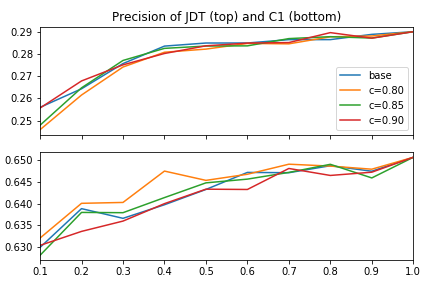
\includegraphics[scale=0.8]{images/Results/RQ1/rq1exp2_Precision.png}
    \caption{Self-training precision when varying fraction of labeled data}
    \label{fig:rq2exp2precision}
\end{figure}

Figure \ref{fig:rq2exp2precision} shows that the precision of all four models is rather similar and it was found that the models do not statistically outperform each other. What is of interest is that the self-trained classifiers achieve similar accuracy when the portion of labelled data is 10\% (hence 90\% being unlabelled) when compared to the accuracy at 100\%. The chosen confidence values do not appear to make a significant difference over one another. The precision values tend to be more similar in the JDT project but experience more fluctuations for the C1 project.

\subsubsection{Recall}

\begin{figure}[H]
    \centering
    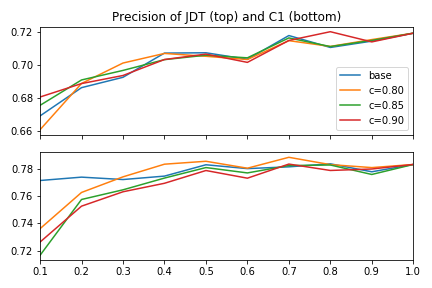
\includegraphics[scale=0.8]{images/Results/RQ1/rq1exp2_Recall.png}
    \caption{Self-training performance when varying fraction of labeled data}
    \label{fig:rq2exp2recall}
\end{figure}

For the C1 project, figure \ref{fig:rq2exp2recall} shows that the recall of the self-trained classifiers bis much lower than that of the base classifier when the fraction of labelled data is between 0.1 and 0.3. However after 0.3, the classifiers recover and achieve similar performance. 

\subsubsection{F1}

\begin{figure}[H]
    \centering
    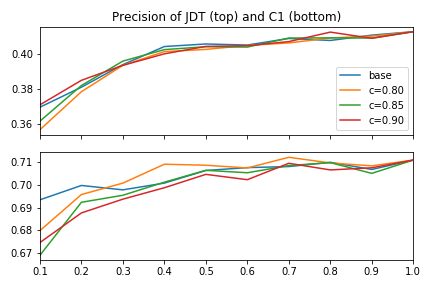
\includegraphics[scale=0.8]{images/Results/RQ1/rq1exp2_F1.png}
    \caption{Self-training performance when varying iterations}
    \label{fig:rq2exp2f1}
\end{figure}

\subsection{Varying the Iterations for Self-Training}

\begin{figure}[H]
    \centering
    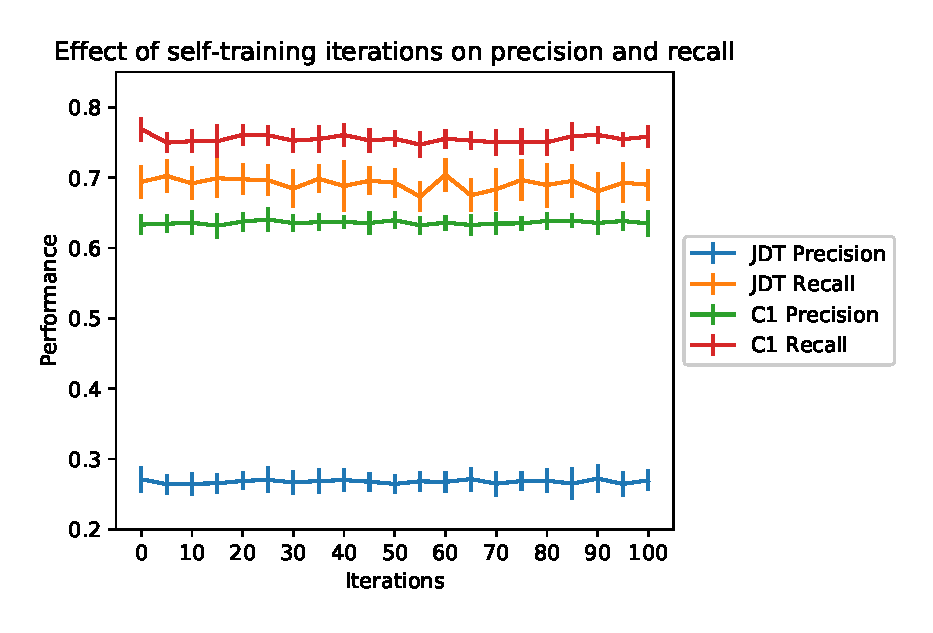
\includegraphics[scale=0.8]{Experiment_3.eps}
    \caption{Self-training performance when varying iterations}
    \label{fig:rq1exp3}
\end{figure}


As seen in figure \ref{fig:rq1exp3}, the precision and recall of the self-trained model does not appear to be affected by the number of iterations. This could indicate that the algorithm stops adding new samples to its training set early on.

\section{Research Question 3 Results}\label{section:rq3exp}

This section shows the results of the case study that was performed (see section \ref{section:case_study}) using 8 members of the C3 project. The model used in this experiment was a random forest model with 100 estimators. This model trained entirely on historical commits for the C3 project and did not use the self-training algorithm. A total of 27 predictions with a label of \textit{not risky} were sent to the developers such that each developer receives a prediction for a commit they created. Then, 20 commits with a label of \textit{risky} were also found using manual inspection of commits within the C3 project. The confusion matrix (see table \ref{table:confusionMatrix}) highlights the performance of this model. 

\begin{table}[H]
    \centering
    \caption{Confusion matrix for trained classifier making live predictions}
    \renewcommand\arraystretch{1.5}
    \setlength\tabcolsep{0pt}
    \begin{tabular}{c >{}r @{\hspace{0.7em}}c @{\hspace{0.4em}}c @{\hspace{0.7em}}l}
    \multirow{10}{*}{\parbox{1.1cm}{\bfseries\raggedleft Predicted\\ label}} & 
    & \multicolumn{2}{c}{\bfseries True label} & \\
    & & \textit{Risky} & \textit{Not Risky} & \bfseries Total \\
    & \textit{Risky} & \MyBox{TP = 6}{} & \MyBox{FP = 5}{} & P$'$ = 11 \\[2.4em]
    & \textit{Not Risky} & \MyBox{FN=14}{} & \MyBox{TN=22}{} & N$'$ = 36\\
    & \textbf{Total} & P = 20 & N = 27 &
    \end{tabular}
    \label{table:confusionMatrix}
\end{table}

\begin{table}[H]
    \centering
    \caption{Performance of trained vs random model}
    \begin{tabular}{|c|c|c|c|} 
    \hline
    \textbf{Metric} & \textbf{Trained Model} & \textbf{Random Model} & \textbf{Cross validation performance}\\ 
    \hline\hline
     Accuracy & 0.596 & 0.500 & 0.835 \\
     Precision & 0.545 & $<$0.545 & 0.639\\
     Recall & 0.300 & 0.500 & 0.778 \\
     F1 & 0.387 & $<$0.387 & 0.702\\
     \hline
    \end{tabular}
    \label{table:rq3Perf}
\end{table}

Table \ref{table:rq3Perf} shows the trained model's performance metrics which are derived from the confusion matrix above. It also shows the performance of a random model as a worst case baseline. Finally, the column \textbf{Cross validation performance} contains the results obtained from the tables \ref{table:rq1_Precision}, \ref{table:rq1_Recall} and \ref{table:rq1_F1} for the exact same project and model. There is a large discrepancy between the performance achieved when evaluating with datasets labelled by the approximate SZZ as opposed evaluating on manually labelled commits. Reasons for this could be that the definition of a risky commit according to developers and to the SZZ algorithm are different. 

\section{Research Question 4 Results}

For this research question, the conducted interviews asked 10 participants a total of 4 questions. All responses are presented in tables such that there is a table for each question asked and each table row contains the response provided by each developer. For each question asked, the results are also summarized as bar plots where the independent axis contains categories for the responses and the dependent axis is the number of responses that associate with this category. Note that a response can fall into more than one category and that the available categories cover all of the responses. Any table row which contains the value \textit{N/A} indicates no applicable response was available for this question. The $i^{th}$ interviewee's response is recorded in the $i^{th}$ row of each table.

\subsection{Interview topic 1: Identifying the Origin of Bugs}

\textit{Once you realize something is faulty with your software, how do you go about locating the origin of the bug ?}

\begin{table}[H]
\centering
\caption{Responses to interview question 1}
    \begin{tabular}{|p{15cm}|}
        \hline
        \textbf{Responses}\\ 
        \hline\hline
        Approach the developers working on the particular project with bugs and see if they know what is wrong. Alternative, I try and guess myself what the cause is. The best way would be to inspect the code.\\
        \hline
        Once something breaks, open up Jenkins and investigate the log which shows any detected failures with the code\\
        \hline
        When a bug occurs in a live product, rely on assistance from the QA team\\
        \hline
        Usually look at the crash logs to see what caused an issue or reach out to other people who may known what's gone wrong. What's tricky is finding bugs when the game runs without crashing but the bugs produce unexpected behaviours. It's more challenging when you don't know which exact system was affected and need a way to narrow it down.\\
        \hline
        Use automation testing and try to see when a buggy commit first appeared. Do this by testing every commit with unit tests\\
        \hline
        Try to reproduce the bug and see what part of the code it belongs to. Use breakpoints and debugging to see why error occurs.\\
        \hline
        Use lots of logs statements when debugging before and after where a potential error or crash occurs\\
        \hline
        Try to reproduce the bug using test cases. Also, use debugging to step through the code.\\
        \hline
        Go through logs to see if the software is behaving normally. I also look at the stack trace as well as previous commits and compare the difference using \texttt{git diff}. It's harder to detect a bug if no crash occurs and the software appears to be running normally. \\
        \hline
        I tend to use the debugger and look at stack traces to see what's wrong. If the program has incorrect behaviour but doesn't crash, I check that individual variables have the correct values. \\
        \hline
    \end{tabular}
\label{table:rq4Table1}
\end{table}

The four categories of responses are \textit{reach out to other  members, inspect logs, detect bug in unit testing} and \textit{manually inspect code with debugger}. The category \textit{reach out to other members} considers responses where verbal communication was required between colleagues, this can include talking to people who do not work with software development. The category \textit{inspect logs} includes looking at stack traces other types of logs. The category \textit{detect bug in unit testing} is for responses which involved finding bugs through test cases. The category \textit{manually inspect code with debugger} is for explicitly setting breakpoints within code and using a debugging tool. 

\begin{figure}[H]
    \centering
    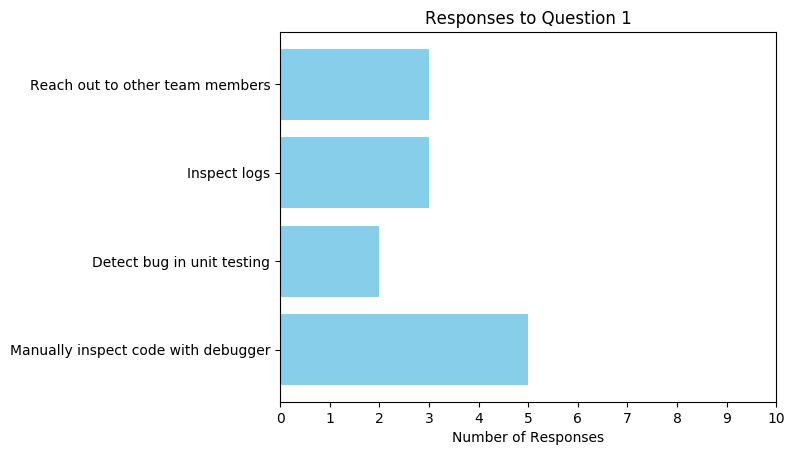
\includegraphics[scale=0.7]{images/Results/RQ2/RQ2_question_1.png}
    \caption{Responses for interview question 1 categorized}
    \label{fig:rq4Image1}
\end{figure}

\subsection{Interview topic 2: Tools Used to Identify and Reduce Bugs}

\textit{What existing tools do you use that help you mitigate the risk of introducing bugs or to help detect bugs?}

\begin{table}[H]
\centering
\caption{Responses to interview question 2}
    \begin{tabular}{|p{15cm}|}
        \hline
        \textbf{Responses}\\ 
        \hline\hline
        I use Trello for planning and communication to ensure people are coordinated\\
        \hline
        Test environments which try to replicate the environment that a live system uses without having to make changes to the live system. Allows you to see if software is working well for various releases and dependency versions\\
        \hline
        Rely on automated unit testing and crash tools that show a stack trace of function calls that failed. I also rely on analytic tools which show the modules that failed and continuous integration servers for regular testing.\\
        \hline
        Use GitHub to see look at differences between commits and understand how they altered the behaviour of code. Also use CppCheck to perform a static analysis of C++ code. Most of my development is done in an integrated development environment (IDE) that provides warnings for common errors. I also use tools that can visualize memory usage to spot memory leaks and linting tools to see if methods are deprecated.\\
        \hline
        Use tools that do static checks, for example verifying that JSON and XML files are valid. Also use GitHub to do pull requests when reviewing code as well as relying on unit tests and manual testing.\\
        \hline
        I do frequent unit testing for the game logic and automatic testing that plays the games to ensure that features work during execution.\\
        \hline
        N/A\\
        \hline
        I rely on unit testing\\
        \hline
        I use the Git merge tool and IDE hints\\
        \hline
        Tools within the IDE that highlight potential errors like SonarLint.\\
        \hline
    \end{tabular}
\label{table:rq4Table2}
\end{table}

\begin{figure}[H]
    \centering
    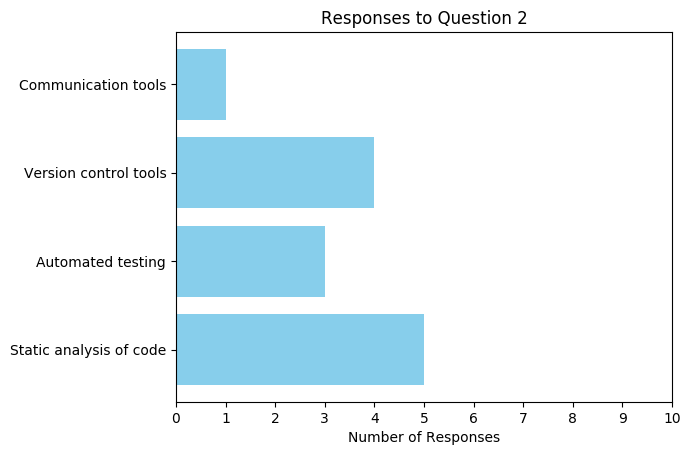
\includegraphics[scale=0.7]{images/Results/RQ2/RQ2_question_2.png}
    \caption{Responses for interview question 2 categorized}
    \label{fig:rq4Image2}
\end{figure}

The four specified categories are \textit{communication tools}, \textit{version control tools}, \textit{automated testing} and \textit{static analysis of code}. 

\subsection{Interview topic 3: Differences Between Clean and Faulty Code}

\textit{What differences do you notice between faulty code and clean code?}

\begin{table}[H]
\centering
\caption{Responses to interview question 3}
    \begin{tabular}{|p{15cm}|}
        \hline
        \textbf{Responses}\\ 
        \hline\hline
        N/A\\
        \hline
        Buggy code tends to be confusing for other developers to understand, its files are too larger and has a lot of dependencies on other files. Also, it's very likely for code to have bugs if there's a lot of nested loops because it makes it more complex for the developer to comprehend\\
        \hline
        N/A\\
        \hline
        Easy to spot if a certain coding practice has been misused, one example is pointers in C++. It's difficult to tell if the code will function correctly if the function calls become very deep.\\
        \hline
        High code complexity such as nested loops and lots of if statements make it hard to understand the code and leads to more bugs.\\
        \hline
        Code that is messy such as having nested loops and being hard to understand tends to have more bugs. Sometimes intuition tells us if certain code is written in an improper manner. \\
        \hline
        Buggy code tends to have hardcoded values and contains a methods that fail to generalize for all possibilities. \\
        \hline
        Code tends to be more buggy when the files are long and when function and variable names are difficult to understand. When code is not easily readable, it becomes harder to debug. Also, buggy code tends to overuse the nesting of loops and if statements.\\
        \hline
        If the code is too complex with lots of if else statements and for loops, makes it harder to read and it makes it harder for programmers to spot bugs. \\
        \hline
        Buggy code is difficult to understand and is poorly documented or the documentation is out of date. It also has a lot of nested loops or nested if statements.\\
        \hline
    \end{tabular}
\label{table:rq4Table3}
\end{table}

\begin{figure}[H]
    \centering
    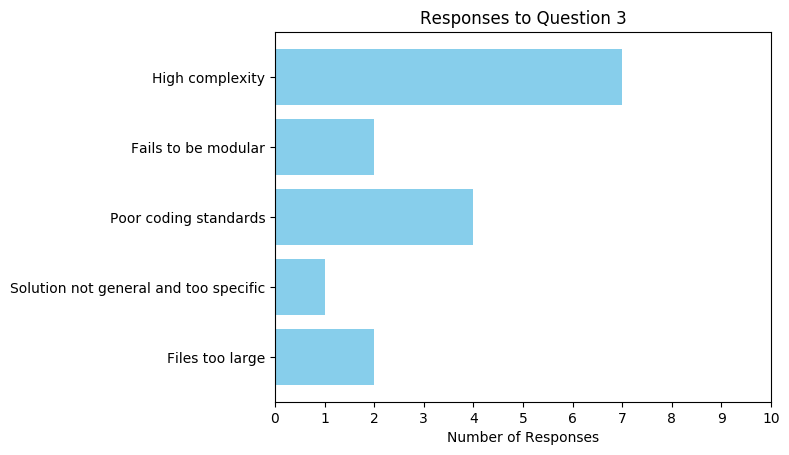
\includegraphics[scale=0.7]{images/Results/RQ2/RQ2_question_3.png}
    \caption{Responses for interview question 3 categorized}
    \label{fig:rq4Image3}
\end{figure}

The five categories for this response are \textit{high complexity}, \textit{failing to be modular}, \textit{poor coding standards}, \textit{solutions not general and too specific} and \textit{files too large}. \textit{High complexity} corresponds to code where it is difficult for a developer to understand what the code does. \textit{Poor coding standards} can involve practices such as having little to no comments, 

\subsection{Interview topic 4: Top Causes for Bugs}

\textit{What do you believe are the top causes of bugs ? }

\begin{table}[H]
\centering
\caption{Responses to interview question 4}
    \begin{tabular}{|p{15cm}|}
        \hline
        \textbf{Responses}\\ 
        \hline\hline
        Lack of resources such as time and money causes development to get rushed.\\
        \hline
        Files that are too large because it's easier for defects to go unnoticed. Also having code that is poorly organized due to too many dependencies and non modular code.\\
        \hline
        Some developers create new code with the assumption that legacy code works properly because it's been given lots of time to fix its bugs. It's also difficult to change legacy code as the fix could lead to more problems than before.\\
        \hline
        Tight deadlines which caused work to be rushed and puts pressure on developers. Sometimes developers put a lot of pressure on themselves, especially when trying to get a new feature released before a holiday. Refactoring code can also a cause a lot of bugs because when refactoring, there is a constraint to ensure the changes don't break the current system.\\
        \hline
        When you get frequently interrupted when doing a task and forget crucial details about the task you were working on.\\
        \hline
        Logical errors that haven't thought of all the possible cases.\\
        \hline
        Tight deadlines which causes developers to write quick solutions that work for now but not in the long term. High complexity within code is also a large contributing factor to causing bugs as well as having developers write code for tasks they are inexperienced with.\\
        \hline
        When code becomes too complex and it's hard to keep track of everything.\\
        \hline
        Temporary solutions that will work for now but not in long term. These solutions fail to generalize and causes technical debt to build up. Also, bugs can arise when files are too long and when code is not modular.\\
        \hline
        When there's a lack of frequent testing and when you have incorrect assumptions about the expected behaviour of a new feature.\\
        \hline
    \end{tabular}
\label{table:rq4Table4}
\end{table}

\textit{Poorly organized code} is the category contains causes such as failing to be modular, having poor documentation or having too many dependencies for example. The category \textit{cognitive state of developers} indicates factors such as stress, external pressure to meet deadlines as well as losing focus as causes of bugs. \textit{Temporary solutions} are for responses where the solution fails to work in the long term. 

\begin{figure}[H]
    \centering
    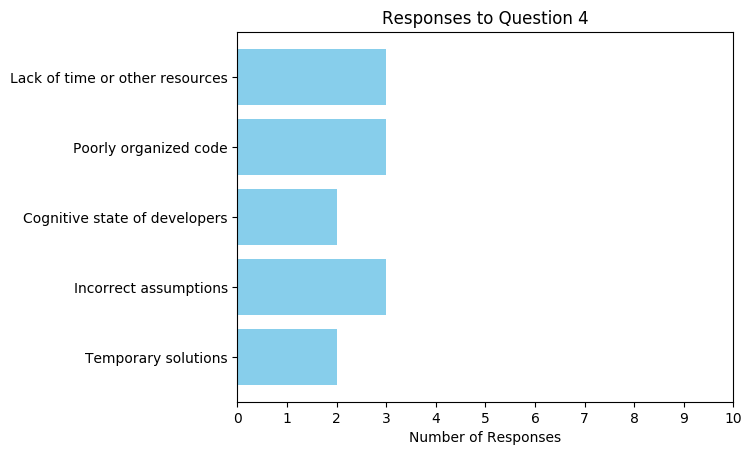
\includegraphics[scale=0.7]{images/Results/RQ2/RQ2_question_4.png}
    \caption{Responses for Question 4 categorized}
    \label{fig:rq4Image4}
\end{figure}

\end{document}